\documentclass{beamer}
\usepackage{amsmath, amssymb}
\usepackage{graphicx}
\usepackage{listings}
\usepackage{color}
\usepackage{subfig}
\usepackage{hyperref}
\usepackage{empheq}
\usepackage{tcolorbox,fancyvrb,xcolor,tikz}
\tcbuselibrary{skins,breakable}

\newenvironment{VerbatimIN}
 {\VerbatimEnvironment
  \begin{tcolorbox}[
    breakable,
    colback=lightgray,
    spartan
  ]%
  \begin{Verbatim}}
 {\end{Verbatim}\end{tcolorbox}}

 \newenvironment{VerbatimOUT}
 {\VerbatimEnvironment
  \begin{tcolorbox}[
    breakable,
    spartan
  ]%
  \begin{Verbatim}}
 {\end{Verbatim}\end{tcolorbox}}

% Set up R code formatting
\definecolor{codegreen}{rgb}{0,0.6,0}
\definecolor{codegray}{rgb}{0.5,0.5,0.5}
\definecolor{codepurple}{rgb}{0.58,0,0.82}
\definecolor{backcolour}{rgb}{0.95,0.95,0.92}
\lstdefinestyle{Rstyle}{
    backgroundcolor=\color{backcolour},
    commentstyle=\color{codegreen},
    keywordstyle=\color{magenta},
    numberstyle=\tiny\color{codegray},
    stringstyle=\color{codepurple},
    basicstyle=\ttfamily\footnotesize,
    breakatwhitespace=false,
    breaklines=true,
    captionpos=b,
    keepspaces=true,
    numbers=left,
    numbersep=5pt,
    showspaces=false,
    showstringspaces=false,
    showtabs=false,
    tabsize=2
}

\title{Mixed Effects Models - Week 8}
\subtitle{Inference in Mixed Effects Models}
\author{Marieke Wesselkamp\\Department of Biometry and Environmental Systems Analysis\\Albert-Ludwigs-University of Freiburg (Germany)}
\date{December 2024}

\begin{document}

\frame{\titlepage}

\begin{frame}
    \frametitle{Hypothesis Testing}
    \large
    A procedure to control the type I error rate $\alpha$. It ensures that we incorrectly reject the null hypothesis (false positive) only with probability $\alpha$. There are four possible outcomes in hypothesis testing:
    \small
    \begin{table}[]
    \begin{tabular}{|l|l|l|}
    \hline
    \textbf{} & \textbf{$H_0$ True} & \textbf{$H_0$ False} \\
    \hline
    $H_0$ No Rejection & Correct 95\%; $p = 1 - \alpha$ & Type II Error 20\%; $p = \beta$ \\
    $H_0$ Rejection & Type I Error 5\%; $p = \alpha$ & Correct 80\%; $p = 1 - \beta$\\
    \hline
    \end{tabular}
    \end{table}
\end{frame}

\begin{frame}
    \frametitle{p-value}
    \large
    The p-value is the probability of obtaining a result equal to or more extreme than the observed data, if the null hypothesis was to be true and the \textbf{appropiate} statistical test was used. \\
    It is not a guarantee that your alternative hypothesis is true, but if the probability was to be small, it is unlikely that the data would have been observed under the null hypothesis.
    \vspace{0.2cm}
\end{frame}

\begin{frame}
\frametitle{}
    \centering
    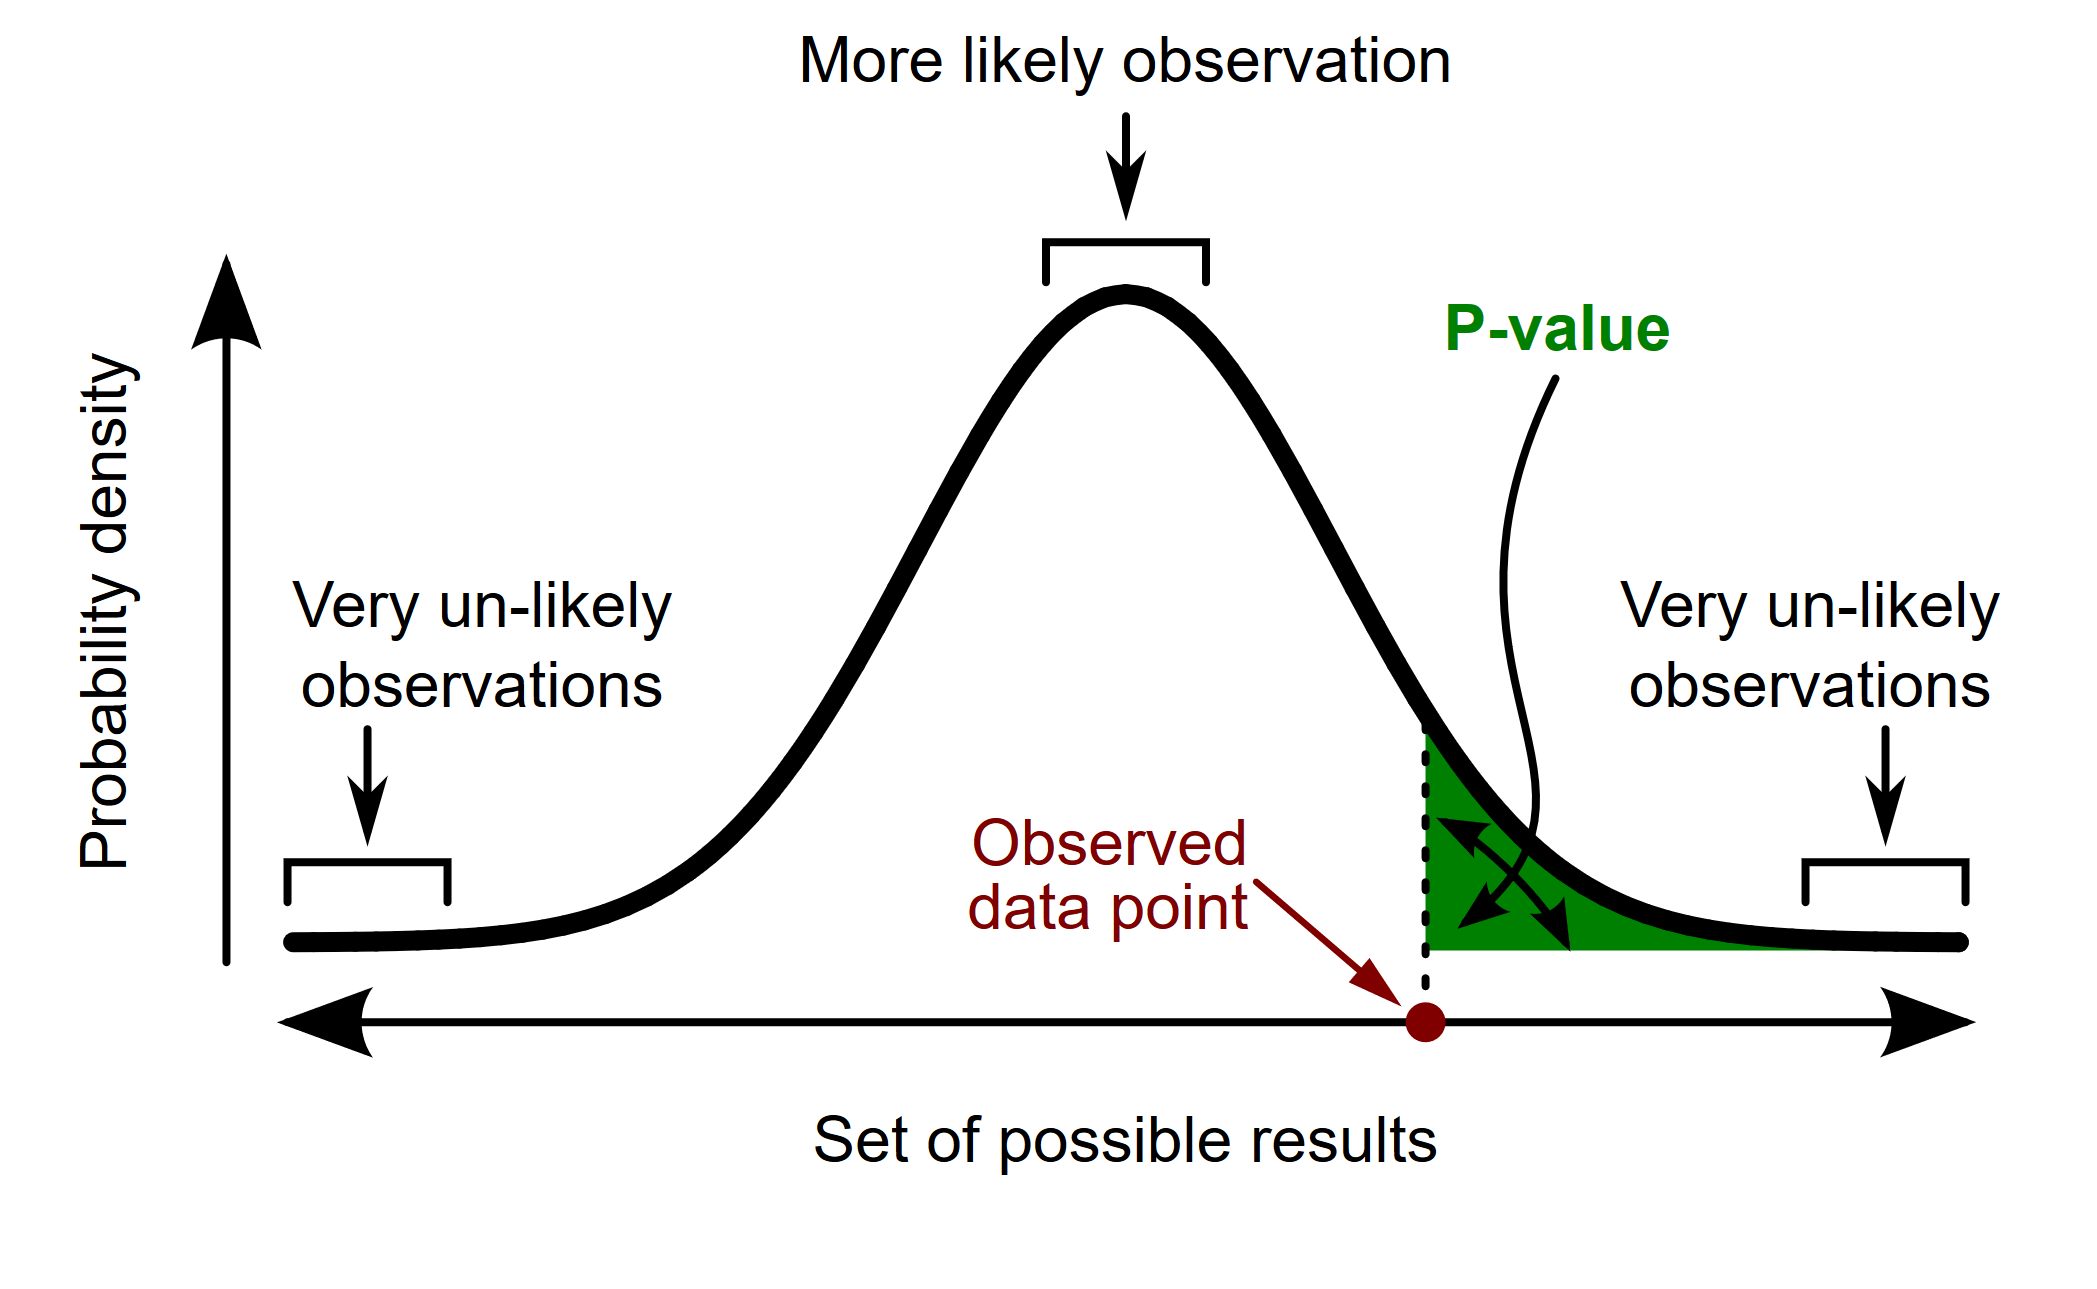
\includegraphics[width=0.9\textwidth]{lectures/day_8_inference_in_mems/figures/p-value.png}
    \begin{itemize}
        \item Small p-value $\Rightarrow$ unlikely data if $H_0$ is true.
        \item Large p-value does not mean $H_0$ is true (power may be low).
    \end{itemize}
\end{frame}

\begin{frame}
\frametitle{Type I \& II Error}
\large
    A significant p-value does not mean that your alternative hypothesis is true:\\
    In 5\% of cases (1 in 20), you commit a Type I error.
    \vspace{0.3cm}
    A large p-value does also not mean that the null hypothesis is true, as the \textbf{power} ($1 - \beta$) of your test may be very low ($\beta$ as the Type II error).

    \small
    \begin{table}[]
    \begin{tabular}{|l|l|l|}
    \hline
    \textbf{} & \textbf{$H_0$ True} & \textbf{$H_0$ False} \\
    \hline
    $H_0$ No Rejection & Correct 95\%; $p = 1 - \alpha$ & Type II Error 20\%; $p = \beta$ \\
    $H_0$ Rejection & Type I Error 5\%; $p = \alpha$ & Correct 80\%; $p = 1 - \beta$\\
    \hline
    \end{tabular}
    \end{table}
\end{frame}

\begin{frame}
    \frametitle{Steps of Hypothesis Testing}
    \begin{enumerate}
        \item Formulate a null hypothesis $H_0$
        \item Formulate an alternative hypothesis $H_A$
        \item Decide on an appropriate test
        \item Check the test assumptions about the sample
        \item Calculate the relevant test statistic of observations
        \item Compare that test statistics to the null distribution and check if the test statistic lies in the critical region (defined by your chosen $\alpha$)
        \item Take the p-value and decide whether you reject your $H_0$ or not (whether you accept $H_A$ or not)
    \end{enumerate}
\end{frame}

\begin{frame}
    \frametitle{Testing Parameters}
    \Large
    In statistical modeling, hypothesis testing often involves testing whether parameters are zero:
    \centering
    \[
    H_0: \beta = 0
    \]
    \textbf{vs.}
    \[
    H_A: \beta \neq 0
    \]
\end{frame}

\begin{frame}
    \frametitle{Issues with Hypothesis Testing}
    \Large
    \begin{itemize}
        \item \textbf{Black-or-white, yes-or-no} attitude in science.
        \item \textbf{Effect size}, \textbf{parameter} estimation, and \textbf{uncertainty} are often overlooked.
        \item Emphasizes \textbf{falsification} once a hypothesis is rejected.
    \end{itemize}
    \vspace{0.3cm}
    Therefore: \textit{Keep it simple and ideally test a single question per dataset.}
\end{frame}

\begin{frame}
    \frametitle{Single vs. Group Parameter Tests}
    \Large
    \textbf{Consider the model:}
    \[
    size_{ij} = \beta_0 + \beta_1 \cdot food + \beta_2 \cdot food^2 + \epsilon_{ij}
    \]
\end{frame}

\begin{frame}
    \frametitle{Single Parameter Test}
    \Large
    \begin{align*}
    &size_{ij} = \beta_0 + \beta_1 \cdot food + \beta_2 \cdot food^2 + \epsilon_{ij}\\
    &size_{ij} = \beta_0 + \beta_1 \cdot food \quad \qquad + \; \qquad \epsilon_{ij}\\
    \\
    &H_0: \beta = 0 \qquad H_A: \beta \neq 0
    \end{align*}
    Testing whether the quadratic term $\beta_2 = 0$. Here, the non-linear (quadratic) effect of food on size equals the t-tests in model summary.
\end{frame}

\begin{frame}
    \frametitle{Group Parameter Test}
    \Large
    \begin{align*}
    &size_{ij} = \beta_0 + \beta_1 \cdot food + \beta_2 \cdot food^2 + \epsilon_{ij}\\
    &size_{ij} = \beta_0 \qquad \qquad \quad + \quad \qquad \qquad \epsilon_{ij}\\
    \\
    &H_0: \beta_1 = \beta_2 = 0 \qquad H_A: \beta_2 \neq 0
    \end{align*}
    Testing whether both $\beta_1 = 0$ and $\beta_2 = 0$ (The complete \textit{food} term). This can be done using an F-test in ANOVA.
\end{frame}

\begin{frame}
    \frametitle{Testing in Mixed Effects Models}
    \Large
    In Mixed Effects Models, you can test:
    \begin{itemize}
        \item Variance components (random effects).
        \item Fixed effects.
    \end{itemize}
\end{frame}

\begin{frame}
    \frametitle{Variance Components}
    \Large
    \textbf{Questions to test:}
    \begin{itemize}
        \item Is there a correlation between a random slope and random intercept?
        \item Is there a random slope?
        \item Is there a random intercept?
    \end{itemize}
\end{frame}

\begin{frame}
    \frametitle{General Advice on Random Effects Testing}
    \large
    \textbf{But:} The general approach to grouped data is to consider \textbf{not} testing the random effects structure. \textbf{Keep it maximal}.
    \vspace{0.2cm}
    
    i.e decide to keep a variance component based on criteria like component size or problematic issues like exactly zero, 1 or -1, instead of deciding based on a p-value.
    \vspace{0.2cm}
    
    \textit{Also: Testing with REML!}
    
\end{frame}

\begin{frame}
    \frametitle{Testing with REML!}
    \textbf{Random intercept vs random slope:}
    \[
    \mathbf{G} = \begin{pmatrix}
    var_{11} & covar_{12} \\
    covar_{21} & var_{22}
    \end{pmatrix}    
    \]
    \begin{align*}
     &H_0: covar_{12} = covar_{21} = 0 \quad or \quad covar_{12} = covar_{21} = var_{22} = 0\\
     &H_A: covar_{12} = covar_{21} \neq 0 \quad or \quad var_{22} \neq 0
    \end{align*}        
    
    Test whether the covariance or variance components are zero.
\end{frame}

\begin{frame}
    \frametitle{Testing Methods}
    \Large
    \begin{itemize}
        \item Likelihood Ratio Test (LRT)
        \item Parametric Bootstrapping
    \end{itemize}
\end{frame}

\begin{frame}
    \frametitle{Log-Likelihood Ratio Test (LRT)}
    Compares two \textbf{nested} models (a more complex and a simpler version) using the difference in their $2 \cdot log-likelihoods$. The result is approximately $\chi^2$ distributed:
    \[
    H_0: var_{22} \neq 0
    \]
    Against the simpler
    \[
    H_1: var_{22} \neq 0
    \]
    The simpler model is a subset of the complex model, which is achieved by setting one or more parameters to zero.
\end{frame}

\begin{frame}[fragile]
\frametitle{Log-Likelihood Ratio Test (LRT)}
\large
\textbf{But: Testing via LRT is not clear-cut.}
\begin{itemize}
    \item It only Approximates. Degrees of freedom are required to calculate LL, but they are not clearly determined for random effects with many levels.
    \item The $\chi^2$ approximation breaks down at boundaries, as a variance component can't be smaller than 0
\end{itemize}
\end{frame}

\begin{frame}
    \frametitle{Parametric Bootstrapping}
    \large
    A Model comparison technique for \textbf{nested} models. It uses both models and...
    \begin{itemize}
        \item ... simulates data from both
        \item ... re-fits the models to the simulated data
        \item ... calculates new LRT values 
        \item ... and obtains the p-value from the distribution of these values.
    \end{itemize}
    \vspace{0.2cm}

    \textit{This is not to be confused with the resampling (and non-parametric) bootstrap}
\end{frame}

\begin{frame}
    \frametitle{Testing Fixed Effects}
    \textbf{Common questions:}
    \begin{itemize}
        \item Is there a linear or nonlinear trend in the data?
        \item Is a variable causing the response?
        \item Is an interaction relevant?
        \item Is there a difference between a single level of a treatment and the rest?
    \end{itemize}
    \vspace{0.2cm}

    Be aware of multiple testing and \textbf{keep it minimal}.\\
    Remember: If possible, use one data set for each question/hypothesis asked.
\end{frame}

\begin{frame}
    \frametitle{Testing with ML!}
    \large
    \begin{empheq}[box=\fbox]{align}
    &size_{ij} = \beta_0 + \beta_1 \cdot food + \beta_2 \cdot food^2 + \epsilon_{ij}\nonumber\\
    \nonumber\\
    &H_0: \beta = 0 \qquad H_A: \beta \neq 0\nonumber 
    \end{empheq}
    \vspace{0.3cm}
    
    \begin{empheq}[box=\fbox]{align}
    &size_{ij} = \beta_0 + \beta_1 \cdot food + \beta_2 \cdot food^2 + \epsilon_{ij}\nonumber\\
    &size_{ij} = \beta_0 \qquad \qquad \quad + \quad \qquad \qquad \epsilon_{ij}\nonumber\\
    \nonumber\\
    &H_0: \beta_1 = \beta_2 = 0 \qquad H_A: \beta_2 \neq 0 \nonumber
    \end{empheq}
\end{frame}

\begin{frame}
    \frametitle{Which Test?}
    \Large
    \textbf{From worst to best:}
    \begin{itemize}
        \item Wald test, F-tests
        \item Likelihood ratio test
        \item F-tests with corrected df (Satterwaithe, Kenwood-Rogers)
        \item Parametric bootstrapping
    \end{itemize}
\end{frame}

\begin{frame}
    \frametitle{Model Selection with Information Criteria}
    \large
    For non-nested models, use an Information Criterion e.g. (corrected) $AIC_c$:
    \[
    AIC_c = -2 \ell + 2 p + \frac{2p(p+1)}{n-p-1}
    \]
    where $\ell$ is the log-likelihood, $p$ is the number of parameters, and $n$ is the sample size.
    \vspace{0.2cm}
    
    \textit{The smaller the $AIC_c$, the better a model}
\end{frame}

\begin{frame}
    \frametitle{Bayesian Information Criterion (BIC)}
    An alternative to AIC: the Bayesian Information Criterion (BIC, with in-built sample size correction)
    \[
    BIC = -2 \ell + p \cdot \log(n)
    \]
     where $\ell$ is the log-likelihood, $p$ is the number of parameters, and $n$ is the sample size.
     \vspace{0.2cm}
     
    \textit{Again: smaller values indicate better models.}
    \vspace{0.2cm}

    \textbf{Information Criteria do not test hypotheses, they compare models!}
\end{frame}

\begin{frame}
    \frametitle{Assessing Model Fit}
    The proportion of total variance explained by a model is given by the coefficient of determination:
    \[
    R^2 = \frac{Var_{Res}}{Var_{Total}} \times 100
    \]
    
    In Mixed Effects Models, different variances can be considered:
    \begin{itemize}
        \item Marginal $R^2$: The variance explained by fixed effects only.
        \item Conditional $R^2$: The variance explained by fixed \textbf{and} random effects.
    \end{itemize}
\end{frame}

\begin{frame}
    \frametitle{Some Literature}
    \large
    \textbf{For Derivation and Limitations see:}\\
    
    \href{https://besjournals.onlinelibrary.wiley.com/doi/full/10.1111/j.2041-210x.2012.00261.x}{Nakagawa, Shinichi, and Holger Schielzeth. "A general and simple method for obtaining R2 from generalized linear mixed‐effects models."} \textit{Methods in ecology and evolution 4.2} (2013)
    \vspace{0.2cm}
    
    \href{https://besjournals.onlinelibrary.wiley.com/doi/full/10.1111/2041-210X.12225}{Johnson, Paul CD. "Extension of Nakagawa \& Schielzeth's R2GLMM to random slopes models."} \textit{Methods in ecology and evolution 5.9} (2014)
\end{frame}

\begin{frame}[fragile]
    \frametitle{Marginal $R^2$ in R}
    How much variance is explained by fixed effects? Check the marginal $R^2$
    \scriptsize
    \begin{VerbatimIN}[numbers=left,numbersep=6pt]
library(lme4)
library(MuMIn)
#performance::r2, MuMin::r.squaredGLMM
r2(mod)
    \end{VerbatimIN}
    \begin{VerbatimOUT}[numbers=left,numbersep=6pt]
# R2 for Mixed Models

  Condirional R2: 0.806
     Marginal R2: 0.409
    \end{VerbatimOUT}
    \begin{VerbatimIN}[numbers=left,numbersep=6pt]
r.squaredGLMM(mod)
    \end{VerbatimIN}
    \begin{VerbatimOUT}[numbers=left,numbersep=6pt]
           R2m       R2c
[1,] 0.4094709 0.8061243
    \end{VerbatimOUT}
\end{frame}

\begin{frame}
    \frametitle{Intraclass Correlation Coefficient (ICC)}
    ICC quantifies the proportion of total variance attributable to group differences:
    \[
    \text{ICC} = \frac{\sigma^2_{group}}{\sigma^2_{group} + \sigma^2_{residual}}
    \]
    ICC for random intercept models equals the variance partitioning coefficient:
    \[
    \text{ICC} = \frac{\sigma^2_{intercept}}{\sigma^2_{intercept} + \sigma^2_{residual}}
    \]
\end{frame}

\begin{frame}[fragile]
    \frametitle{ICC for Inspection of random components in R}
    \scriptsize
    \begin{VerbatimIN}[numbers=left,numbersep=6pt]
mod <- lmer(distance ~ age*Sex + (age | Subject), data = Orthodont)
    \end{VerbatimIN}
        \begin{columns}
        \begin{column}{0.6\textwidth}
        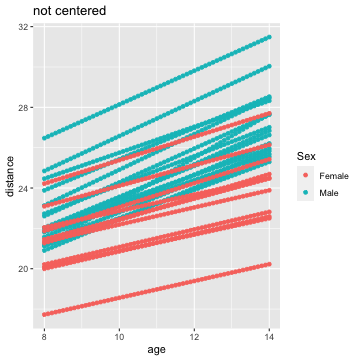
\includegraphics[width=\textwidth]{lectures/day_8_inference_in_mems/figures/unnamed-chunk-5-1.png}
        \end{column}
        \begin{column}{0.4\textwidth}
            \large What proportion of the total variance is attributable to differences among groups?
        \end{column}
    \end{columns}
\end{frame}

\begin{frame}[fragile]
\frametitle{ICC with and without Random Slope?}
    \begin{columns}
        \begin{column}{0.55\textwidth}
        \tiny
            \begin{VerbatimIN}[numbers=left,numbersep=6pt]
mod <- 
lmer(distance ~ age*Sex + (age|Subject), 
data = Orthodont)
VarCorr(mod)                
            \end{VerbatimIN}
            \begin{VerbatimOUT}[numbers=left,numbersep=6pt]
 Groups   Name        Std.Dev. Corr  
 Subject  (Intercept) 2.40302        
          age         0.18014  -0.667
 Residual             1.31020 
            \end{VerbatimOUT}
            \begin{VerbatimIN}[numbers=left,numbersep=6pt]
icc(mod)
            \end{VerbatimIN}
            \begin{VerbatimOUT}[numbers=left,numbersep=6pt]
# Intraclass Correlation Coefficient

     Adjusted ICC: 0.672
  Conditional ICC: 0.397
            \end{VerbatimOUT}
            \begin{VerbatimIN}[numbers=left,numbersep=6pt]
(2.40^2 + 0.18^2)/(2.40^2 + 0.18^2 + 1.31^2)
            \end{VerbatimIN}
            \begin{VerbatimOUT}[numbers=left,numbersep=6pt]
[1] 0.7714457
            \end{VerbatimOUT}
        \end{column}
        \begin{column}{0.55\textwidth}
                    \tiny
            \begin{VerbatimIN}[numbers=left,numbersep=6pt]
mod2 <- 
lmer(distance ~ age*Sex + (1|Subject), 
data = Orthodont)
VarCorr(mod2)               
            \end{VerbatimIN}
            \begin{VerbatimOUT}[numbers=left,numbersep=6pt]
 Groups   Name        Std.Dev.
 Subject  (Intercept) 1.8162  
 Residual             1.3864 
 
            \end{VerbatimOUT}
            \begin{VerbatimIN}[numbers=left,numbersep=6pt]
icc(mod2)
            \end{VerbatimIN}
            \begin{VerbatimOUT}[numbers=left,numbersep=6pt]
# Intraclass Correlation Coefficient

     Adjusted ICC: 0.632
  Conditional ICC: 0.373
            \end{VerbatimOUT}
            \begin{VerbatimIN}[numbers=left,numbersep=6pt]
(1.81^2)/(1.81^2 + 1.38^2)
            \end{VerbatimIN}
            \begin{VerbatimOUT}[numbers=left,numbersep=6pt]
[1] 0.6323907
            \end{VerbatimOUT}
        \end{column}
    \end{columns}
\end{frame}

\begin{frame}[fragile]
\frametitle{}#
\large
\textbf{Wait a minute! This doesn't yield the same results...}
    \begin{columns}
        \begin{column}{0.55\textwidth}
        \tiny
            \begin{VerbatimOUT}[numbers=left,numbersep=6pt]
# Intraclass Correlation Coefficient

     Adjusted ICC: 0.672
  Conditional ICC: 0.397
            \end{VerbatimOUT}
            \begin{VerbatimIN}[numbers=left,numbersep=6pt]
(2.40^2 + 0.18^2)/(2.40^2 + 0.18^2 + 1.31^2)
            \end{VerbatimIN}
            \begin{VerbatimOUT}[numbers=left,numbersep=6pt]
[1] 0.7714457
            \end{VerbatimOUT}
        \end{column}
        \begin{column}{0.55\textwidth}
                    \tiny
            \begin{VerbatimOUT}[numbers=left,numbersep=6pt]
# Intraclass Correlation Coefficient

     Adjusted ICC: 0.632
  Conditional ICC: 0.373
            \end{VerbatimOUT}
            \begin{VerbatimIN}[numbers=left,numbersep=6pt]
(1.81^2)/(1.81^2 + 1.38^2)
            \end{VerbatimIN}
            \begin{VerbatimOUT}[numbers=left,numbersep=6pt]
[1] 0.6323907
            \end{VerbatimOUT}
        \end{column}
    \end{columns}
    \vspace{0.3cm}

    \large
\textbf{Only for the random intercept model}, the ICC equals the partioning coefficient
\end{frame}

\begin{frame}
    \frametitle{}
    \large
    \textbf{Useful and convinient packages:}
    \begin{itemize}
        \item For summary stats: `performance`, `MuMIn`, `afex`
        \item For ICC: `performance`
        \item For model comparison: `lmerTest` (After Satterwaithe)
        \item For plotting: `performance`, `interplot` 
    \end{itemize}
    \vspace{0.2cm}

    \textit{Be aware that things constantly change, contain partial contradictions and sometimes use different definitions. It is often difficult to find out how things are really calculated.}
\end{frame}

\begin{frame}
    \frametitle{Recapitulation Day 9}
    \large
    \textbf{Topics covered today:}
    \begin{itemize}
        \item What and what not (AICc, BIC) \textbf{hypothesis testing} is \textbf{single} vs. \textbf{group} parameter tests
        \item Hypothesis testing on \textbf{variance components}
        \item Hypothesis testing on \textbf{fixed effects} in LMEMs
        \item When to use REML or ML
    \end{itemize}
    \vspace{0.2cm}
    
    Afternoon Exercises: Inference in LMEMs
\end{frame}

\end{document}